\subsection{Flow Engineering}
\label{s:floweng}

\begin{figure}
\centering
%\begin{minipage}{.45\textwidth}
  \centering
  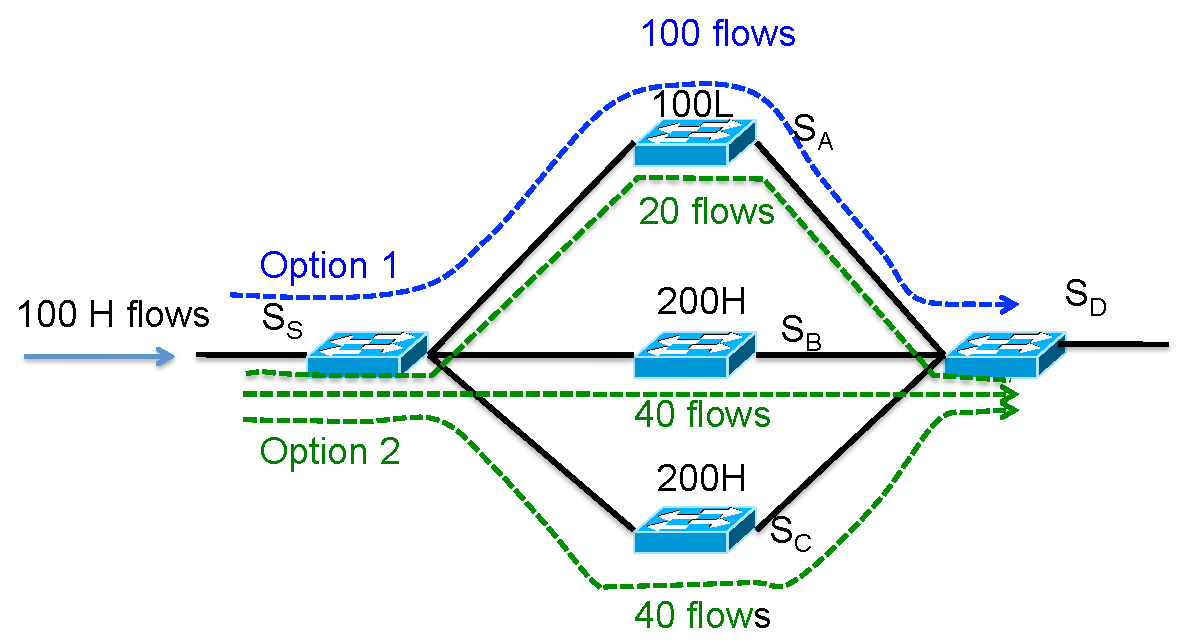
\includegraphics[width=3.2in]{figs/flow_eng_example.pdf} \compactcaption{Flow 
engineering example, assuming \BroadcomOne. $nL$ = $n$ low priority rules;
$nH$ = $n$ high priority rules; capacity = 1000 rules. Ingress and egress 
tables are empty} 
\label{fig:flow_eng} \end{figure}

SDN applications that perform failure recovery, traffic engineering, or other
forms of routing must quickly compute and setup network paths in order to
satisfy reachability and performance objectives. These applications must often
select one of many possible paths based on congestion, delay, flow table 
occupancy, or other metrics. Unfortunately, a (slightly) more optimal path 
according to these metrics may take significantly longer to setup due to 
outbound latency.

For example, consider an SDN application that seeks to minimize the
imbalance in flow table occupancy~\cite{swan, simple, minlanvcrib}. If such an
application needed to setup routes for 100 flows of high priority $H$ in the
topology shown in Figure~\ref{fig:flow_eng}, it would select the first path
through switch $S_A$ for all flows, thereby equalizing the number of flow
table entries across all switches. However, assuming the switches are
\BroadcomOne, this would require displacing {\em each} of the 100 existing
rules of low priority $L$ in $S_A$ for {\em each} of the 100 new flows,
resulting in a total flow installation time of $\approx$1.5s. In contrast, by
routing only 20 new flows through $S_A$, and dividing the remaining flows
evenly between the paths through $S_B$ and $S_C$, we can keep the same level
of imbalance in flow table occupancy ($S_B$ and $S_C$ each have twice as many
entries as $S_A$), while reducing the total flow installation time to
$\approx$0.3s (assuming rules are installed in $S_A$, $S_B$, and $S_C$ in
parallel). 


%SDN applications typically compute paths between various network
%locations that meet some global objective pertaining to
%performance or security. A common issue considered in most prior works
%on such applications is to deal with limited switch table sizes, by
%picking routes that obey or optimize table space
%constraints~\cite{swan,simple, minlanvcrib}. Unfortunately,
%these techniques do not provide sufficient control over outbound
%delay. 

%\minisection{Minimize maximum flow table occupancy is very suboptimal} 
%For example, consider a simple setting where there are three candidate
%paths between a pair of nodes as shown in Figure~\ref{fig:flow_eng}.
%Each path has one Broadcom switch. The switch on the first path
%has 100 rules of low priority L, whereas the switches on the second
%and third paths each have 400 rules of high priority H. Suppose that a
%hypothetical traffic engineering application has 100 flows of priority
%H to allocate to these paths, and each path is equally preferable
%for a flow.  Existing techniques for table space management would
%assign all flows to the first path to minimize maximum flow table occupancy; but
%our measurements for Broadcom 
%show that {\em each} of these 100 rules will displace
%all the 100 low priority rules in the TCAM, resulting in high
%latencies! Allocating 50 flows each on the
%latter two paths instead results in no rule displacement, and the number of
%rules installed per path will be smaller. Thus, when the flows are installed in
%parallel across the latter two paths, this results in significant reduction in
%installation latency. Based on Figure~\ref{fig:burst-completion-time}, it is about 200 ms
%vs 2 seconds, a 10X difference. 
%%Intel switches have similar issues, but for other priority patterns.
%%li: yes, according Marina's information. Low priority rule displaces high
%%priority rule depending on their location.
%%\aditya{check intel claim}

The goal of {\em flow engineering} (\FE) is to select paths that minimize
installation delay while still satisfying an SDN application's primary path
selection criteria (e.g., flow table occupancy or congestion). Assuming there
are many possible sets of paths $\{\mathcal{P}^i_{obj}\}_i$ that (closely)
satisfy an application's objectives, FE selects the set
$\mathcal{P}^{displace}_{obj,tbl\_sz}$ that minimizes the aggregate
latency impact of rule installations, and any associated rule displacements,
while still obeying flow table space constraints.
%The goal of flow engineering is to select paths across the network
%such that installation delay is minimized. The key insight we use is
%the following: in general, there are many possible sets of paths
%$\{\mathcal{P}^i_{obj}\}_i$ in a network that optimize an SDN
%application's objectives, e.g., optimal capacity and latency. From
%this, flow engineering selects the set
%$\mathcal{P}^{displace}_{obj,tbl\_sz}$ that minimizes the aggregate
%impact of both rule displacement in TCAM as well as the number of rules
%installed at any switch, while obeying table space constraints.
% maximum number of rules installed at any
% switch; thus, we spread rule update load {\em laterally}, helping
% improve outbound latencies.
%
$\mathcal{P}^{displace}_{obj,tbl\_sz}$ can be computed using a two step
optimization:
({\em i}) identify sets of paths that satisfy the SDN application's objective 
function,
%\aaron{What is ``the network's objective function?''}
but do not select the actual
paths to use; ({\em ii}) select paths that minimize aggregate
flow installation time.
%effect of rule displacement and the number of rules to be inserted at any
%switch.  
Unfortunately, the time required to solve the integer linear program
(presented in  \appref{app:floweng}) would
outweigh the latency benefits it seeks provide, so we formulate an
efficient heuristic.
%The detailed optimization formulation is a large integer linear
%program (omitted for brevity) and hence inefficient to solve. Below, we
%discuss a simplifying heuristic in the context of a traffic engineering
%application.

\minisection{Flow Engineering Heuristic}
Our goal is to satisfy a bound $C$ on the time required to install/modify
rules across all switches. 
%We initialize $C$ to a low value.

We represent the network as a graph $G = (V,E)$, where each node is a switch
(or PoP) and each edge is a link (or tunnel). Given a traffic matrix $M$, the
SDN application computes $K$ candidate equal cost paths for each $(u,v) \in
V$, where cost is defined in terms of the application's objective (e.g.,
average link utilization). We assume the application also assigns a priority
$Pri(u,v)$ to each flow $(u,v)$.

%\aaron{This is very specific to the objective of minimizing average link
%utilization; can we make this more generic?} 

We sort the flows in decreasing order of resource demand (e.g., bandwidth) and
iterate through them. For each flow $(u,v)$ in the sorted order, we consider
the corresponding $K$ equal cost paths in decreasing order of resource 
availability; let $P^{1\ldots K}_{(u,v)}$ be the sorted order. If the resource
demand $d_{uv}$ can be satisfied by the path $P^{1}_{(u,v)}$, then we compute
whether installing/updating rules for flow $(u,v)$ along this path violates the
latency bound $C$.

%We do this by modeling the per-switch latency, as well as maximum latency
%on the path:

%We represent the network as a graph \textit{G = (V,E)}, where each node is a
%switch (or PoP) and each edge is a link (or tunnel). Given
%a traffic matrix $M$, the application attempts to route it such that the
%average link utilization is within some bound; the heuristic can be easily
%extended to accommodate other objectives.
%% Our goal to compute routes such that the objective is maximized as well as
%% the cost of installing the necessary rules at switches is minimized. 
%%Our heuristic works by exploring for each source-destination pair
%For each source-destination pair we see, whether a path can accommodate both
%its demand, and the path setup latency  
%%imposed by routing the pair across the path's switches 
%is within some bound. If either is violated, we try the next candidate path.
%
%More precisely, suppose we want to bound the maximum cost of
%installing rules at any switch by some $C$. We start by selecting some
%low value for $C$. We assume that we have computed $K$ candidate equal cost
%paths for each $(u,v) \in V$. Suppose the priority of the $(u,v)$ flow
%is $Pri(u,v)$ at every switch in the network (this is
%typically set by the operator).
%
%We sort the traffic demands in decreasing order and
%iterate through them. For each $(u,v)$ in the sorted order, we
%consider the corresponding $K$ equal cost paths in decreasing order
%of available capacity; let $P^{1\ldots K}_{(u,v)}$ be the sorted order. 
%
%If the demand $d_{uv}$ can be satisfied by the path $P^{1}_{(u,v)}$ within
%the utilization bound, then we compute whether installing the $(u,v)$ path
%violates the rule installation latency bound or not. We do this by modeling
%the per-switch latency, as well as maximum latency on the path:



%\minisection{Per-switch latency}
% Recall that we always install new rules,
%and never do rule modifications and deletions. 
%\aditya{the previous sentence may have to go}
% In doing this, an issue to consider is whether the rule for
% $(u,v)$ at $s$ is modifying an existing forwarding rule for $(u,v)$ at
% $s$ (this would happen if $(u,v)$ was being routed through $s$ before,
% but the next hop from $s$ has now changed) or it is a new rule being
% inserted (this happens if $(u,v)$ was never routed via $s$ before).
% However, recall that our measurements show that modifying a rule is
% much more expensive than inserting a new rule (the former incurs the
% cost of potentially reshuffling the entire existing set of rules at
% the switch, whereas the latter only displaces lower priority rules).
% Therefore, we {\em always insert} a new rule for $(u,v)$, ensuring
% that the rule is of higher priority than the existing rule for $(u,v)$
% in $s$ (if any). 
Given our measurement results, for every switch $s \in P^{1}_{(u,v)}$, we can
model the latency at $s$ due to installing rules for $(u,v)$ as 
$L_s = \max(a, (b +c * Disp_s(Pri(u,v))))$. Here, $Disp_s(Pri(u,v))$ is the 
number of rules at $s$ that will be displaced by the rule for $(u,v)$.
%% the following discussion is not very useful, it seems 
%For the Broadcom switch, this is the number of rules of priority {\em lower}  than $Pri(u,v)$, whereas for the Intel switch
%$Disp_s(Pri(u,v))$ is the number of rules of priority \emph{higher} than
%$Pri(u,v)$ divided by 300. 
%This is a conservative estimate assuming all rules
%are packed in increasing priority of slices (\S\ref{s:meas_insert}).
%\aditya{check intel claim} 
%$Disp_s(Pri(u,v))$ can be easily tracked by the SDN
%controller. In the above, 
$a$, $b$ and $c$ are constants derived from switch
measurements. This model essentially says that if the current rule
does not displace any rules from $s$'s existing table, then it incurs
a fixed cost of $a$; otherwise, it incurs the cost given by $b +c *
Disp_s(Pri(u,v))$. The fixed cost $a$ is the insertion delay without any TCAM
reordering. 

%$a$ is the same whether it is modification or insertion for Intel. For
%Broadcom, since we avoided modification, it represents insertion delay without
%TCAM displacement. 
%\aditya{refer back to the model from
%  the measurement section}

%\minisection{Maximum installation latency} 
Now, $\forall s \in P^{1}_{(u,v)}$, we check if $L_s + CurrentL_s \le C$,
where $CurrentL_s$ is the current running total cost of installing the
rules at $s$, accumulated from vertex pairs considered prior to $(u,v)$ in our
iterative approach.
If this inequality is satisfied, we assign $(u,v)$ to the path
$P^{1}_{(u,v)}$ and move to the next vertex pair. If not,
%meaning that installing the $(u,v)$ route on this path violates the
%maximum cost bound $C$ for some switch on the path, then 
we move to the next candidate path for $(u,v)$, i.e., $P^{2}_{(u,v)}$ and
repeat the process.

If after iterating through all flows once, we have not selected a feasible
path for each flow, then we increase $C$ and start from the beginning.
Alternately, we could do a simple binary search on $C$. 
%li: no space for that.
%\aditya{do we need pseudocode?}

%\aditya{assumption: we have a small number of rules we are adding.
%  otherwise, if we can confirm that the decreasing priority weirdness
%  does not apply for all table occupancies, then we should use that}
%\aditya{seems like bcm is buggy so we may not need the above
%  assumption}

% We assign each edge a cost that is the reciprocal of its current available capacity, and find the 
% minimum cost path for the traffic demand. For finding the minimum cost path, we consider precomputed K equal hop length paths, and find
% the path which gives the minimum cost. As we assign a path for a particular traffic demand, 
% we reassign the cost by decreasing the current capacity by the traffic demand for each edge belonging to the
% min-cost path. The idea is that edges which are more highly utilized will get a higher cost value and so the min-cost path for remaining 
% traffic demands will prefer the edges which are lightly utilized. This way, 
% we minimize the maximum load. We analyze the runtime complexity of the algorithm. 

% 
\begin{table}
\begin{scriptsize}
\begin{tabular}{c|l}
Notation & Meaning \\
\hline
$S$ & Set of all switches
\\$S_{ToR}$ & Set of all ToR switches
\\$\tau_{u}$ & Maximum number of flow entries in the switch $u \forall u \in S$
\\$E$ & Set of all physical links (between two adjacent devices)
\\$C_e$ & capacity of individual links $\forall e \in E$
\\$F_{uv}$ & set of all flows from $u$ to $v$ where $u,v \in S$
\\$P_{uv}$ & Set of paths from device $u$ to device $v$
\\$K _{uv}$ & Number of paths from device $u$ to $v$ where $u,v \in S$ 
\\$P^k _{uv}$ & Set of links of $k^{th}$ path from device $u$ to $v$ where $u,v \in S$
\\$T ^f _{uv}$ & Traffic volume from $u$ to $v$ of flow $f$ where $u,v \in S$
\\$util$ & maximum link utilization
\\$I ^{fk} _{uv}$ & Indicator variable denoting that flow $f$ from $u$ to $v$  takes the $k^{th}$ path.
\\$cost$ & maximum cost of rule installation at any switch
\\$M$ & priority of all new rules being inserted
\\$L_s(M)$ & number of rules at switch $s$ of priority lower than $M$
\\ $a$ & cost of installing a rule it has same priority as rules in table
\\ $b$ & constant factor used in modeling rule displacement cost.
\end{tabular}
\label{tab:notation1}
\caption{Notation used in flow engineering formulation.}
\end{scriptsize}
\end{table}

We explain how flow engineering works for simple traffic engineering SDN
application. We represent
the network as a graph \textit{G
  = (V,E)}, where each node is a switch (or a PoP) and each edge is a physical link (or virtual tunnel). Given a traffic matrix, the application attempts to route it such that the maximum link utilization is minimized. Upon computing routes, the application determines the rules to be installed at individual switches. 

For simplicity, we assume that all the rules to be inserted are of the same priority $M$.  We also assume that the control application knows how many rules in each switch have priority lower than $M$, i.e., $L_s(M)$. This can be easily tracked based on history of rule insertions. The notation we use is shown in Table~\ref{tab:notation1}.


{\bf Step 1 - Network Objective:} In the first step we minimize the
maximum link utilization. Let $T ^f _{uv}$ be the traffic volume
 of flow \textit{f} between $(u,v)$, $P^k _{uv}$ be the set of links on
the $k^{th}$ path between (\textit{u,v}). We use a
binary indicator variable $I ^{fk} _{uv}$ to show whether the flow $f$
is on path $k$ or not.  $K _{uv}$ denotes the number of equal hop
length paths between $(u,v)$. 

We have the following capacity constraint: 

% Following are our two
% constraints. First, The total traffic volume from an edge should not
% exceed its $C_e$ times the link utilization limit, $util$. 

\begin{scriptsize}	
\begin{equation*}
    \sum _{u,v \in S_{ToR},~f \in F_{uv},~k  \in P_{uv}~s.t.~e \in P^k _{uv}} T ^f _{uv} *  I^{fk}_{uv} \leq util \times C_e 
\end{equation*}
\end{scriptsize}	
	
The following ensures each flow $f$ takes a single path:	

\begin{equation*}
    \sum _{k  \in P_{uv}} I^{fk}_{uv} = 1 ,\quad \quad \forall u,v \in S_{ToR},~ f \in F_{uv}
\end{equation*}
 
The objective is to minimize the \textit{util}. Note that we do not
compute paths in this step, just the value of the objective function;
suppose the optimal value is $util^*$.

{\bf Step 2 - New Rule Objective:} In second step, we select routes
so as to minimize the rule installation latencies at any
switch. We allow some slack wrt meeting the utilization objective; denote it by
$\delta$. While the second constraint above remains, the capacity
constraint changes to:
 
% First,  traffic traversing from an edge $e$ does not exceed the $C_e$ multipled by 1 $+$ $\delta$ times the $util^*$. $util^*$ is the maximum link utilization we got from the step 1, and  $\delta$ defines an upper limit on maximum link utilization.

\begin{scriptsize}
\begin{equation*}
    \sum _{u,v \in S_{ToR},~f \in F_{uv},~k  \in P_{uv}~s.t.~e \in P^k _{uv}} T ^f _{uv} *  I^{fk}_{uv} \leq (1 + \delta) \times util^* \times C_e 
\end{equation*}
\end{scriptsize}

% We have a similar constraint as above for   Second constraint is same as step 1.\\
  
% \begin{equation*}
%       \sum _{k  \in P_{uv}} I^{fk}_{uv} = 1 ,\quad \quad \forall u,v \in S_{ToR},~ f \in F_{uv}
% \end{equation*}
 % \begin{alignat*}{2}
  %                     & latency = a * entries + c \\
   %                    \text{   where }a \text{ and }c\text{ are constant}\\ 
  %\end{alignat*}

When a rule installed at a switch cause existing lower priority rules to be displaced, we incur a cost that grows linearly with the number of displaced rules, i.e., $b * L_s(M)$, where $b$ is a constant. This cost adds up linearly when a burst of rules is installed. When the burst of rules installed all have the same priority as rules already in the table, we incur a smaller fixed cost per rule, denoted by $a$. Based on this, we track the total cost of rule installation at a switch as follows:
%  for each rule installed at the switch, we incur a cost of we incur a co
% here, we assign a weight ``$a$'' to the number of rules installed and a weight ``$b$'' to the number of rules that need rearrangement:
\aditya{need to make sure we have justification for
  this linear function. provide constants based on measurements.}

\begin{scriptsize}
\begin{equation*}
                       \sum_{u,v \in S_{ToR}, ~f \in F_{uv}, ~k \in
                         P_{uv} ~s.t.~ s\in P^k_{uv} } max(a, b * L_s(M)) I^{fk}_{uv}  +
                       \leq cost \quad \quad \forall s \in S
\end{equation*}
\end{scriptsize}

The objective is to minimize $cost$.   
  



% This can be viewed as solving the following two optimization problems
% in sequence:

% \[
% \begin{array}{lll}
% \text{Problem 1:} & \text{optimize} & NetworkObjective \\
% & \text{subject to} & RuleCapacities \\
% \end{array}
% \]

% \[
% \begin{array}{lll} 
% \text{Problem 2:} & \text{optimize} & NewRuleObjective \\
% & \text{subject to} & NetworkObjective \text{, and, } \\
% & & RuleCapacities
% \end{array}
% \]

% Here $NetworkObjective$ is the SDN application's network wide
% objective function, such as maximum link utilization, $RuleCapacities$
% represent switch table capacities in the network, and
% $NewRuleObjective$ an objective function pertaining to new rules
% inserted at any switch, such as the maximum number of such rules. The
% first optimization problem simply computes the value of the objective
% function, e.g. the maximum link utilization, subject to switch table
% capacity constraints; no actual paths are computed. The second
% optimization problem uses this value as a constraint to compute
% $P^{flowmod}_{obj,tablesize}$.

\minisection{Limitations} Because paths are computed by the SDN application, FE
must be integrated with the application. FE does not apply to scenarios where 
route updates are confined to a single location, presenting no opportunity to
spread update load laterally. One such example is MicroTE~\cite{microte},
where changes in traffic demands are accommodated by altering rules at the
source ToR to reallocate ToR-to-ToR flows across different tunnels.

\iffalse
{\bf Interaction with Update Semantics:}
Flow engineering has to be designed carefully when
management applications are trying to realize various consistency
properties for their updates~\cite{mahajan13:hotnets}. We explain
using examples below.

If updates of network state from ``old'' to ``new'' are not
orchestrated carefully, a variety of consistency issues can arise:
e.g., there may be forwarding loops, or packets may be forwarded
inconsistently (using old state some times and new state at other
times) at different network hops. Both issues are transient, and flow
engineering (as well as the rule offloading and priority ordering
techniques we describe below) can reduce the duration of such loops
by bounding the time that any network switch spends updating
its state.

In practice, some network operators may want to ensure some semantics
for their updates. One example is packet
coherence~\cite{mahajan13:hotnets}, which means
a packet should see consistent state (always old, or always new) as it
traverses the network. This can be achieved using global version
numbers and one-shot updates~\cite{consistentupdates}: (a) new
forwarding state is added to the core of the network, keeping older
state around; (b) the edge is updated to use the new state only when
all core switches confirm the installation of the new state; prior to
this all forwarding happens using old state; (c) old state is removed
from the network only when there are no more packets forwarded using
it. Flow engineering as formulated above directly helps in this case
by speeding up step (a). 

Consider another example semantics, loop freedom; this can be achieved
by ensuring that switches downstream on a new forwarding path are
updated, and their new state used for forwarding, before those
upstream~\cite{mahajan13:hotnets}. In this case, naively applying flow
engineering as specified above may hurt: because it may increase the
number of switches and paths being updated it may correspondingly
increase the aggregate number of ``dependencies'' to track amongst
different switches' updates, slowing down loop-free updates.
Furthermore, spreading of updates across multiple paths can also
introduce dependency cycles; expensive mechanisms are necessary to
break these cycles~\cite{mahajan13:hotnets}. which further slow down
the update. Thus, the total latency of doing a loop-free update can be
significantly higher with naive flow engineering.

We must therefore design appropriate flow engineering schemes for
different update protocols. We leave a full exploration of this issue
for future work. Where the issue arise, we assume the network is using
one-shot updates.

\aditya{lead out}

\fi

%\subsubsection{MicroTE}

% LocalWords:  Broadcom SDN TCAM rearrangment tbl sz PoP Pri uv Disp CurrentL
% LocalWords:  MicroTE ToR
